\documentclass[11pt,a4paper]{article}

\usepackage[utf8]{inputenc}
\usepackage[T1]{fontenc}
\usepackage[spanish,es-nodecimaldot]{babel}
\usepackage{lmodern}
\usepackage{geometry}
\usepackage{xcolor}
\usepackage{graphicx}
\usepackage{hyperref}
\usepackage{enumitem}
\usepackage{listings}
\usepackage{longtable}
\usepackage{tabularx}
\usepackage{booktabs}
\usepackage{fancyhdr}
\usepackage{microtype}
\usepackage{float}
\usepackage{caption}

\geometry{top=2.1cm,bottom=2.1cm,left=2.2cm,right=2.2cm}
\graphicspath{{docs/assets/tutorial-2026-10-09/}}
\hypersetup{
  colorlinks=true,
  linkcolor=blue!55!black,
  urlcolor=blue!60!black,
  pdftitle={Bitácora práctica del bootstrap Azure Databricks Dev},
  pdfauthor={Proyecto Databricks CI/CD}
}

\definecolor{dbblue}{HTML}{1B4F72}
\definecolor{dbcyan}{HTML}{117A8B}
\definecolor{dbgreen}{HTML}{287D3C}
\definecolor{dborange}{HTML}{B45F06}
\definecolor{lightblue}{HTML}{EAF2F8}
\definecolor{lightgreen}{HTML}{EAF5EC}
\definecolor{lightorange}{HTML}{FFF3E6}
\definecolor{codebg}{HTML}{F6F8FA}
\definecolor{codegray}{HTML}{586069}

\pagestyle{fancy}
\fancyhf{}
\lhead{Proyecto Azure Databricks CI/CD}
\rhead{Bitácora práctica - Dev}
\cfoot{\thepage}
\setlength{\headheight}{14pt}

\setlist[itemize]{leftmargin=1.4em,itemsep=0.25em,topsep=0.4em}
\setlist[enumerate]{leftmargin=1.6em,itemsep=0.35em,topsep=0.4em}
\setlength{\parindent}{0pt}
\setlength{\parskip}{0.55em}

\lstdefinestyle{projectcode}{
  backgroundcolor=\color{codebg},
  basicstyle=\ttfamily\small,
  breaklines=true,
  columns=fullflexible,
  commentstyle=\color{codegray},
  frame=single,
  framerule=0.3pt,
  rulecolor=\color{black!20},
  showstringspaces=false,
  tabsize=2
}
\lstset{style=projectcode}

\newcommand{\concepto}[1]{\textcolor{dbblue}{\textbf{#1}}}
\newcommand{\resultado}[1]{\colorbox{lightgreen}{\strut\textbf{#1}}}
\newcommand{\atencion}[1]{\colorbox{lightorange}{\strut\textbf{#1}}}
\newenvironment{aprendizaje}{
  \begin{quote}\color{dbblue}\textbf{Concepto clave.}\ }{
  \end{quote}}
\newenvironment{seguridad}{
  \begin{quote}\color{dborange}\textbf{Seguridad.}\ }{
  \end{quote}}

\begin{document}
\hypersetup{pageanchor=false}

\begin{titlepage}
  \centering
  \vspace*{1.8cm}
  {\color{dbblue}\rule{\textwidth}{1.2pt}}\\[0.9cm]
  {\Huge\bfseries Bitácora práctica\\[0.25cm]
  Bootstrap seguro de Azure Databricks Dev\par}
  \vspace{0.65cm}
  {\Large Azure, Terraform, Unity Catalog, identidades y OIDC\par}
  \vspace{0.9cm}
  {\color{dbblue}\rule{\textwidth}{1.2pt}}\\[1.3cm]
  {\large Tutorial reproducible de la sesión de implementación\par}
  \vfill
  \begin{tabular}{rl}
    Proyecto: & \texttt{proyecto-databricks-cicd} \\
    Entorno: & Dev \\
    Región: & East US 2 (\texttt{eastus2}) \\
    Fecha de la sesión: & 9 de octubre de 2026 \\
    Presupuesto mensual: & USD 58 (aprox. S/200) \\
  \end{tabular}
  \vfill
  {\small Los identificadores se muestran truncados y no se incluyen códigos de acceso, tokens ni
  datos personales. Git y Terraform continúan siendo la fuente de verdad.}
\end{titlepage}

\hypersetup{pageanchor=true}
\pagenumbering{roman}
\begingroup
  \small
  \setlength{\parskip}{0pt}
  \tableofcontents
\endgroup
\newpage
\pagenumbering{arabic}

\section{Resultado de la jornada}

La sesión terminó con un entorno Dev funcional y administrado por Terraform. Azure contiene un
Resource Group y un workspace Azure Databricks Premium; Databricks contiene la identidad CI/CD,
la política OIDC para GitHub, el grupo de desarrolladores, las carpetas del proyecto y un esquema
aislado de Unity Catalog. El último \texttt{terraform plan} de ambas capas informó
\texttt{No changes}.

\begin{center}
  \resultado{Estado final: infraestructura creada, reconciliada y sin cómputo activo}
\end{center}

\begin{tabularx}{\textwidth}{@{}p{0.28\textwidth}X@{}}
\toprule
\textbf{Componente} & \textbf{Resultado confirmado} \\
\midrule
Suscripción Azure & Pay-As-You-Go activa y presupuesto mensual de USD 58. \\
Azure Databricks & Workspace \texttt{dbw-databricks-cicd-dev} en \texttt{eastus2}. \\
Terraform Azure & Resource Group y workspace bajo estado local; plan estable. \\
Terraform Databricks & Service principal, OIDC, grupo, permisos, carpetas y esquema; plan estable. \\
Unity Catalog & Catálogo administrado del workspace y esquema \texttt{cicd}. \\
Costo al cierre & Clúster registrado detenido, SQL warehouse detenido y sin jobs activos. \\
\bottomrule
\end{tabularx}

\subsection{Arquitectura lograda}

\begin{lstlisting}
GitHub (futuro workflow con OIDC)
        |
        v
sp-dbx-cicd-dev
        |
        +--> /Workspace/data/proyecto_test        (codigo desplegado)
        +--> /Workspace/.cicd/proyecto_test/dev   (estado protegido)
        +--> catalogo_del_workspace.cicd          (pruebas del pipeline)

Azure subscription
        +--> rg-databricks-cicd-dev
                 +--> dbw-databricks-cicd-dev
\end{lstlisting}

La automatización de GitHub todavía no fue activada. Lo realizado hoy prepara el destino y la
identidad a la que el workflow se autenticará sin Personal Access Tokens.

\section{Modelo mental: dos capas de Terraform}

El laboratorio separa dos responsabilidades para que los cambios sean pequeños y comprensibles:

\begin{enumerate}
  \item \textbf{Capa Azure} (\texttt{infra/azure/dev}): crea recursos de Azure, como el Resource
  Group y el workspace.
  \item \textbf{Capa Databricks} (\texttt{infra/databricks/dev}): usa un workspace ya existente y
  crea objetos internos, identidades, permisos y gobierno de datos.
\end{enumerate}

\begin{aprendizaje}
Un \concepto{provider} enseña a Terraform a hablar con una API. Un \concepto{resource} describe un
objeto que Terraform administra. Una \concepto{variable} introduce un valor configurable, un
\concepto{output} publica un resultado no sensible y el \concepto{state} vincula el código con los
objetos reales. \texttt{plan} propone; \texttt{apply} modifica; \texttt{destroy} elimina.
\end{aprendizaje}

El estado es local durante esta primera fase didáctica. Los archivos \texttt{terraform.tfstate},
\texttt{*.tfplan} y \texttt{terraform.tfvars} están excluidos de Git. Antes de incorporar QA se
migrará el estado a un backend remoto con bloqueo y control de acceso.

\section{Paso 1: suscripción y control de costos}

\subsection{Activación de Pay-As-You-Go}

Se convirtió la cuenta inicial a Pay-As-You-Go y se creó la suscripción
\texttt{Azure\_Databricks\_CICD\_Lab}. La suscripción quedó en estado \textit{Active}. La cuenta
personal que creó la suscripción conserva el rol Owner y se usa para las operaciones de Azure.

El nombre de la suscripción sirve para reconocer el laboratorio; no cambia la seguridad ni el
precio. El identificador real de la suscripción se trató como configuración local y en este
documento se representa como \texttt{ba527c78-...-94dd}.

\subsection{Presupuesto y alertas}

Se creó manualmente el presupuesto \texttt{budget-proyecto-databricks-dev} con estas propiedades:

\begin{itemize}
  \item importe: USD 58 por mes, equivalente aproximado al objetivo de S/200;
  \item reinicio mensual;
  \item alertas de costo real al 50\%, 75\%, 90\% y 100\%;
  \item destinatarios de correo configurados por el propietario.
\end{itemize}

\begin{seguridad}
Un presupuesto \textbf{no detiene} recursos cuando se alcanza el límite. Envía alertas. Para una
respuesta automática haría falta un Action Group y una automatización cuidadosamente diseñada.
Por ahora, el control efectivo es apagar cómputo, revisar Cost Analysis y mantener recursos
efímeros.
\end{seguridad}

El presupuesto ya creado en el portal no se duplicó desde Terraform. La administración del budget
mediante código quedó desactivada para esta fase.

\section{Paso 2: Azure CLI, tenant y MFA}

\subsection{Primer inicio de sesión}

El primer \texttt{az login} respondió con \texttt{AADSTS50076}: Azure exigía autenticación
multifactor por un cambio de política o de ubicación. No era un error de contraseña; significaba
que el flujo necesitaba interacción adicional.

La solución fue especificar el tenant y usar Device Code:

\begin{lstlisting}[language=bash]
az login `
  --tenant "<TENANT_ID>" `
  --use-device-code

az account set --subscription "<SUBSCRIPTION_ID>"

az account show `
  --query "{name:name, id:id, state:state, tenantId:tenantId}" `
  --output table
\end{lstlisting}

La salida esperada mostró la suscripción del laboratorio en estado \texttt{Enabled} y el tenant
correcto. Los códigos de Device Code son temporales y nunca deben copiarse a documentación o Git.

\subsection{Dos identidades con propósitos distintos}

Durante el bootstrap se usaron dos contextos:

\begin{itemize}
  \item \textbf{Cuenta propietaria de Azure}: ve la suscripción y ejecuta Terraform sobre Azure.
  \item \textbf{Usuario organizacional de Entra}: entra al Account Console de Databricks y ejecuta
  el bootstrap de objetos a nivel de cuenta.
\end{itemize}

El usuario organizacional apareció como cuenta a nivel de tenant sin suscripciones. Eso es correcto:
no necesita ser Owner de Azure para administrar temporalmente el Account Console de Databricks.

\section{Paso 3: región y aprovisionamiento del workspace}

Se revisaron las regiones disponibles y se eligió \texttt{eastus2}. La decisión priorizó
disponibilidad del servicio y opciones de cómputo modernas. El costo exacto se evaluará con uso real,
porque depende del tipo y duración del cómputo, no sólo de la región.

\subsection{Variables de Azure}

El archivo local \texttt{infra/azure/dev/terraform.tfvars} contiene nombres, región, tags y el ID de
suscripción. No contiene contraseñas ni tokens y no debe versionarse.

\begin{lstlisting}[language=bash]
subscription_id = "<SUBSCRIPTION_ID>"
location        = "eastus2"
owner           = "<OWNER_TAG>"
\end{lstlisting}

Los tags aplicados fueron \texttt{project}, \texttt{environment}, \texttt{owner} y
\texttt{managed\_by=terraform}. Permiten identificar costos y responsabilidad.

\subsection{Plan revisado}

Como Terraform no estaba instalado globalmente, se utilizó el binario descargado dentro de la
carpeta de caché del proyecto:

\begin{lstlisting}[language=bash]
& ".\.cache\terraform-1.13.4\terraform.exe" `
  -chdir="infra/azure/dev" `
  plan -input=false
\end{lstlisting}

El plan propuso exactamente dos recursos:

\begin{lstlisting}
Plan: 2 to add, 0 to change, 0 to destroy.

+ azurerm_resource_group.this
+ azurerm_databricks_workspace.this
\end{lstlisting}

Se revisaron nombre, región, SKU Premium, Managed Resource Group y tags antes de autorizar el
\texttt{apply}. Después del aprovisionamiento se confirmó el workspace en el portal y un nuevo plan
informó:

\begin{lstlisting}
No changes. Your infrastructure matches the configuration.
\end{lstlisting}

\begin{aprendizaje}
Un plan estable demuestra \concepto{idempotencia}: ejecutar de nuevo la misma definición no propone
duplicados. También detecta drift si alguien modifica manualmente un recurso administrado.
\end{aprendizaje}

\section{Paso 4: acceso administrativo a Databricks}

\subsection{Por qué falló la cuenta personal}

El enlace del Account Console rechazó la cuenta personal de Microsoft con
\texttt{AADSTS500200}. La aplicación esperaba una identidad organizacional de Microsoft Entra ID.
Además, el primer intento de usar un correo sugerido falló porque ese usuario todavía no existía.

La corrección fue crear explícitamente un usuario organizacional llamado
\textit{Databricks Lab Admin} en el tenant y asignarle temporalmente el rol Global Administrator.
Ese rol permitió completar el bootstrap inicial del Account Console.

\begin{figure}[H]
  \centering
  \IfFileExists{docs/assets/tutorial-2026-10-09/entra-global-admin.png}{%
    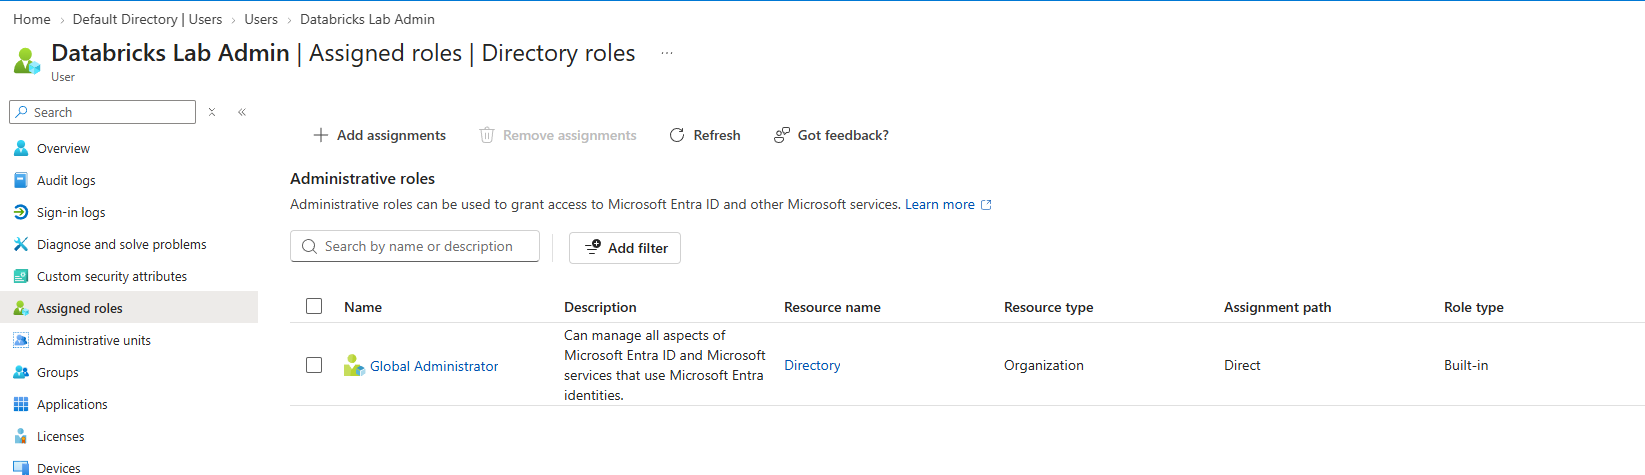
\includegraphics[width=\textwidth]{docs/assets/tutorial-2026-10-09/entra-global-admin.png}%
  }{%
    \fbox{\parbox{0.92\textwidth}{Captura disponible en
    \texttt{docs/assets/tutorial-2026-10-09/entra-global-admin.png}.}}%
  }
  \caption{Rol temporal Global Administrator asignado al usuario organizacional del laboratorio.}
\end{figure}

\begin{seguridad}
Global Administrator es un rol extremadamente privilegiado. Ya no es necesario para el trabajo
cotidiano del laboratorio. Debe retirarse al finalizar el bootstrap y conservarse únicamente el
acceso específico requerido en Databricks.
\end{seguridad}

\subsection{Alta en el workspace}

El usuario organizacional se agregó al workspace con los entitlements necesarios para administrarlo
durante el bootstrap. Se mantuvieron desactivadas la creación irrestricta de clústeres y la creación
de pools.

\begin{figure}[H]
  \centering
  \IfFileExists{docs/assets/tutorial-2026-10-09/databricks-workspace-entitlements.png}{%
    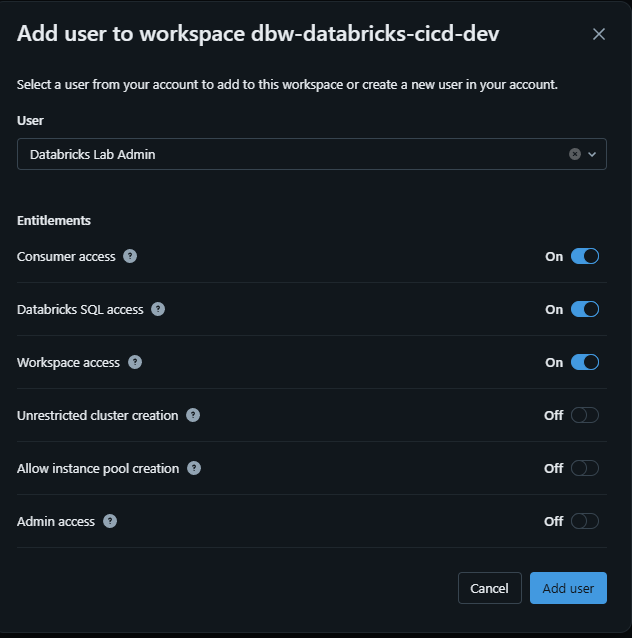
\includegraphics[width=0.70\textwidth]{docs/assets/tutorial-2026-10-09/databricks-workspace-entitlements.png}%
  }{%
    \fbox{\parbox{0.70\textwidth}{Captura disponible en
    \texttt{docs/assets/tutorial-2026-10-09/databricks-workspace-entitlements.png}.}}%
  }
  \caption{Entitlements usados para agregar el usuario administrativo al workspace.}
\end{figure}

Esta separación es importante: un rol de directorio de Entra no equivale a un entitlement o permiso
dentro de Databricks.

\section{Paso 5: configuración Terraform de Databricks}

\subsection{Datos locales y nomenclatura correcta}

Se completó \texttt{infra/databricks/dev/terraform.tfvars} con:

\begin{itemize}
  \item Account ID de Databricks, representado aquí como \texttt{96099a08-...-8274};
  \item Workspace ID y host producidos por la capa Azure;
  \item propietario GitHub \texttt{dbernalesv};
  \item nombre de repositorio \texttt{proyecto-databricks-cicd};
  \item usuario de desarrollo y grupo \texttt{data-engineers};
  \item catálogo administrado asociado al workspace.
\end{itemize}

La variable \texttt{github\_repository} recibe sólo el nombre, no la URL completa. Terraform arma
el subject OIDC con esta forma:

\begin{lstlisting}
repo:<GITHUB_OWNER>/<GITHUB_REPOSITORY>:environment:dev
\end{lstlisting}

Por eso el valor correcto es \texttt{proyecto-databricks-cicd}, mientras que
\texttt{github\_owner} es \texttt{dbernalesv}.

\subsection{Identidad CI/CD y OIDC}

Terraform creó el service principal \texttt{sp-dbx-cicd-dev}. Su Application ID se tratará como
variable de GitHub y se representa aquí como \texttt{89693b08-...-86fe}.

La política de federación confía únicamente en tokens emitidos por GitHub Actions para el repositorio
y el Environment \texttt{dev} exactos. El audience es el Account ID de Databricks.

\begin{aprendizaje}
OIDC intercambia un token de corta duración por acceso durante el job. No hay un PAT permanente que
guardar o rotar. Para funcionar de forma segura, GitHub debe conceder \texttt{id-token: write} sólo
al job de despliegue y el Environment debe estar protegido.
\end{aprendizaje}

\subsection{Grupo y carpetas}

Terraform administra el grupo de cuenta \texttt{data-engineers}, agrega al usuario de desarrollo y
lo asigna al workspace. Los permisos resultantes son:

\begin{tabularx}{\textwidth}{@{}p{0.43\textwidth}p{0.23\textwidth}X@{}}
\toprule
\textbf{Objeto} & \textbf{Principal} & \textbf{Permiso} \\
\midrule
\texttt{/Workspace/data/proyecto\_test} & \texttt{data-engineers} & \texttt{CAN\_EDIT} \\
\texttt{/Workspace/data/proyecto\_test} & Service principal CI/CD & \texttt{CAN\_MANAGE} \\
\texttt{/Workspace/.cicd/proyecto\_test/dev} & Service principal CI/CD & \texttt{CAN\_MANAGE} \\
\bottomrule
\end{tabularx}

Dev permite edición manual para debugging. Sin embargo, el siguiente despliegue reconstruirá la
carpeta desde el SHA de Git y eliminará archivos que no estén en el manifiesto. Los cambios manuales
nunca se promueven a QA o Prod.

\section{Paso 6: Unity Catalog y recuperación del primer apply}

\subsection{Fallo observado}

El primer \texttt{terraform apply} avanzó lo suficiente para crear identidades, grupo y carpetas,
pero falló al intentar crear un catálogo adicional. El workspace nuevo usaba
\textit{Default Storage} y no exponía una raíz de metastore válida para ese catálogo extra.

Este fallo no implicó borrar lo creado. Terraform registró en el state cada recurso confirmado y el
siguiente plan calculó sólo lo pendiente.

\subsection{Decisión adoptada}

Se inspeccionó el workspace y se encontró el catálogo administrado creado automáticamente, respaldado
por Default Storage. En vez de forzar almacenamiento adicional, la configuración se corrigió para:

\begin{enumerate}
  \item leer el catálogo existente con un \texttt{data source};
  \item crear dentro de él el esquema \texttt{cicd};
  \item conceder al service principal \texttt{USE\_CATALOG};
  \item conceder en el esquema \texttt{USE\_SCHEMA}, \texttt{CREATE\_TABLE}, \texttt{MODIFY} y
  \texttt{SELECT}.
\end{enumerate}

La decisión está registrada en \texttt{docs/adr/0005-workspace-catalog-default-storage.md}. El apply
de recuperación completó los objetos pendientes y el plan final volvió a ser estable:

\begin{lstlisting}
No changes. Your infrastructure matches the configuration.
\end{lstlisting}

\begin{aprendizaje}
Este caso muestra por qué no se debe improvisar borrando state o recursos después de un fallo.
Terraform es transaccional por recurso, no por ejecución completa: conserva lo que la API confirmó y
permite reanudar después de corregir la causa.
\end{aprendizaje}

\section{Verificación de costos al cerrar la sesión}

Antes de terminar se consultaron las APIs de Databricks con un token temporal obtenido desde Azure
CLI. No se imprimió el token. El resumen fue:

\begin{lstlisting}
Clusters registrados:          1
Clusters en ejecucion:         0
SQL warehouses registrados:   1
SQL warehouses en ejecucion:  0
Jobs activos:                  0
\end{lstlisting}

El clúster y el SQL warehouse registrados están detenidos. No hay que eliminarlos esta noche para
evitar gasto de cómputo. Tampoco es necesario destruir el workspace o el Resource Group: hacerlo
eliminaría el avance y obligaría a repetir el bootstrap.

\subsection{Qué sí puede facturarse}

Azure Databricks factura principalmente DBUs y máquinas virtuales mientras el cómputo está activo.
También pueden existir cargos pequeños por almacenamiento administrado, disco, red o direcciones
públicas. Con el cómputo detenido, no se espera un consumo horario alto, pero el costo real debe
confirmarse en Cost Analysis porque la facturación puede tener retraso.

\subsection{Lista de cierre seguro}

Al finalizar cada laboratorio:

\begin{enumerate}
  \item abrir \textbf{Compute} y comprobar que todos los clústeres estén \texttt{TERMINATED};
  \item abrir \textbf{SQL Warehouses} y comprobar que estén \texttt{STOPPED};
  \item revisar \textbf{Jobs \& Pipelines} y confirmar que no haya runs activos;
  \item evitar crear endpoints de serving, pools o recursos de red permanentes sin presupuesto;
  \item revisar \textbf{Cost Management > Cost Analysis} al día siguiente;
  \item recordar que las alertas de budget no detienen el consumo.
\end{enumerate}

Para clústeres interactivos futuros se configurará auto-termination. Para jobs se preferirá cómputo
efímero o serverless, siempre con límites y timeouts.

\section{Seguridad pendiente inmediata}

La acción recomendada al retomar el proyecto es retirar el rol \textbf{Global Administrator} del
usuario \textit{Databricks Lab Admin}. El bootstrap ya concluyó. Este cambio no elimina el usuario,
el workspace, el service principal ni la configuración Terraform; reduce el riesgo de una cuenta
innecesariamente privilegiada.

También deben mantenerse estas reglas:

\begin{itemize}
  \item no subir \texttt{terraform.tfvars}, state, planes, tokens ni archivos \texttt{.env};
  \item no copiar tokens de Azure CLI a variables de GitHub;
  \item usar variables de GitHub Environment para IDs y hosts no secretos;
  \item usar OIDC para credenciales efímeras;
  \item no ejecutar workflows de PR no confiables con \texttt{id-token: write}.
\end{itemize}

\section{Qué continúa en la próxima sesión}

La infraestructura base ya no es el bloqueo. El siguiente tramo es conectar GitHub con Dev:

\begin{enumerate}
  \item retirar el rol Global Administrator temporal;
  \item crear o completar el GitHub Environment \texttt{dev};
  \item cargar como variables el host, Account ID y Client/Application ID, sin secretos persistentes;
  \item proteger \texttt{main} con Pull Requests y checks obligatorios;
  \item ejecutar \texttt{validate-pr.yml} y corregir cualquier validación;
  \item probar el login OIDC desde GitHub Actions;
  \item desplegar el Bundle a \texttt{/Workspace/data/proyecto\_test};
  \item ejecutar el smoke test y confirmar el SHA desplegado;
  \item revisar Cost Analysis después de la primera ejecución serverless.
\end{enumerate}

QA y Prod permanecerán sin crear hasta que Dev despliegue de extremo a extremo de forma repetible.

\section{Comandos de diagnóstico reutilizables}

\subsection{Azure}

\begin{lstlisting}[language=bash]
az account show `
  --query "{name:name, id:id, state:state, tenantId:tenantId}" `
  --output table

az resource list `
  --resource-group "rg-databricks-cicd-dev" `
  --output table
\end{lstlisting}

\subsection{Terraform Azure}

\begin{lstlisting}[language=bash]
$tf = ".\.cache\terraform-1.13.4\terraform.exe"

& $tf -chdir="infra/azure/dev" fmt -check
& $tf -chdir="infra/azure/dev" validate
& $tf -chdir="infra/azure/dev" plan -input=false
\end{lstlisting}

\subsection{Terraform Databricks}

Antes de usar la capa Databricks hay que iniciar sesión con el usuario organizacional del tenant y
obtener acceso a la aplicación Azure Databricks. Nunca se debe imprimir el token.

\begin{lstlisting}[language=bash]
az login `
  --tenant "<TENANT_ID>" `
  --use-device-code `
  --allow-no-subscriptions

az account get-access-token `
  --resource "2ff814a6-3304-4ab8-85cb-cd0e6f879c1d" `
  --output none

& $tf -chdir="infra/databricks/dev" fmt -check
& $tf -chdir="infra/databricks/dev" validate
& $tf -chdir="infra/databricks/dev" plan -input=false
\end{lstlisting}

\begin{seguridad}
No ejecutar \texttt{terraform destroy} como rutina de apagado. \texttt{destroy} elimina recursos y
requiere revisar el objetivo exacto. Para controlar el gasto diario basta con detener cómputo. La
destrucción del laboratorio se reservará para una decisión explícita y un plan revisado.
\end{seguridad}

\section{Referencias oficiales}

\begin{itemize}
  \item \href{https://azure.microsoft.com/pricing/details/databricks/}%
  {Microsoft Azure: precios de Azure Databricks}.
  \item \href{https://learn.microsoft.com/azure/cost-management-billing/costs/tutorial-acm-create-budgets}%
  {Microsoft Learn: crear y administrar presupuestos de Azure}.
  \item \href{https://learn.microsoft.com/azure/databricks/compute/configure}%
  {Microsoft Learn: configuración y auto-termination de cómputo}.
  \item \href{https://learn.microsoft.com/cli/azure/authenticate-azure-cli}%
  {Microsoft Learn: autenticación de Azure CLI}.
\end{itemize}

\section*{Conclusión}
\addcontentsline{toc}{section}{Conclusión}

La jornada no terminó únicamente con un workspace visible: terminó con infraestructura declarativa,
identidad CI/CD sin secretos persistentes, permisos explícitos, un esquema aislado y evidencia de
idempotencia. El entorno puede permanecer creado durante la noche porque su cómputo está detenido.
La prioridad al regresar es reducir el privilegio del usuario de bootstrap y conectar GitHub Actions
por OIDC para realizar el primer despliegue reproducible hacia Dev.

\end{document}
